\documentclass{beamer}
\beamertemplatenavigationsymbolsempty
\usepackage{amsmath, amssymb, hyperref, graphics}
\usepackage{tikz}
%\usepackage{mathpazo}
\usetikzlibrary{graphs}
\usetikzlibrary{graphs.standard}


\newcommand{\Z}{\mathbb{Z}}
\newcommand{\Q}{\mathbb{Q}}
\newcommand{\R}{\mathbb{R}}


\title{Graph Theory Lecture 3}




\begin{document}
\begin{frame}{Which graphs are/aren't isomorphic?  Prove it.}
  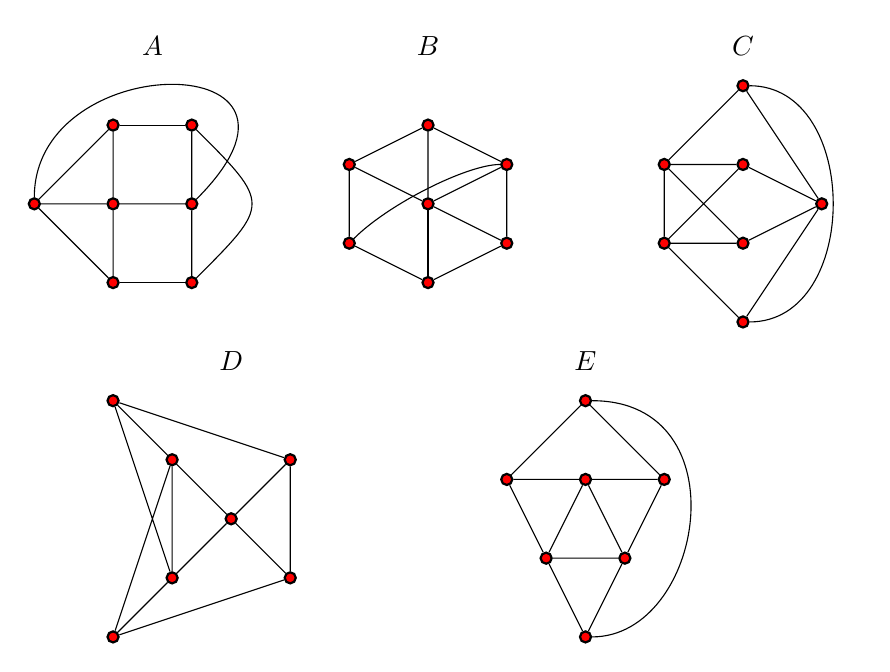
\begin{tikzpicture}
\node at (1.5,2) {$A$};
\node at (5,2) {$B$};
\node at (9,2) {$C$};
\node at (2.5, -2) {$D$};
\node at (7, -2) {$E$};
  \begin{scope}[every node/.style={circle, draw, fill=red, inner sep=0pt, minimum width=4pt, thick}]

    
  \node (a) at (0,0) {};
  \node (b) at (1,1) {};
  \node (c) at (1,0) {};
  \node (d) at (1,-1)  {};
  \node (e) at (2,1) {};
  \node (f) at (2,0) {};
  \node (g) at (2,-1) {};

  \draw (a) -- (b) -- (c) -- (d) -- (a) -- (c) -- (f) -- (e) .. controls (3,0) and (3,0) .. (g)--(f) .. controls (4,2) and (0,2) .. (a);
  \draw (b)--(e);
  \draw (d)--(g);
  

  \begin{scope}[xshift=4cm, scale=.5]
  \node (a) at (0,1) {};
  \node (b) at (0,-1) {};
  \node (c) at (2,2) {};
  \node (d) at (2,0)  {};
  \node (e) at (2,-2) {};
  \node (f) at (4,1) {};
  \node (g) at (4,-1) {};

\draw (b)--(a)--(c)--(f)--(g)--(e)--(b) .. controls (1,0) and (3,1) .. (f)--(d)--(g);
\draw (a)--(d)--(c);
\draw (d)--(e);

    \end{scope}
  
  \begin{scope}[xshift=8cm, scale=.5]
  \node (a) at (0,1) {};
  \node (b) at (0,-1) {};
  \node (c) at (2,3) {};
  \node (d) at (2,1)  {};
  \node (e) at (2,-1) {};
  \node (f) at (2,-3) {};
  \node (g) at (4,0) {};

  \draw (a)--(c) .. controls (5,3) and (5, -3) .. (f)--(b)--(a)--(d)--(b)--(e)--(a);
  \draw (c)--(g)--(d);
  \draw (e)--(g)--(f);

    \end{scope}

  \begin{scope}[yshift=-4cm, xshift=1cm, scale=.75]
  \node (a) at (0,2) {};
  \node (b) at (0,-2) {};
  \node (c) at (3,1) {};
  \node (d) at (3,-1)  {};
  \node (e) at (1,1) {};
  \node (f) at (1,-1) {};
  \node (g) at (2,0) {};

  \draw(a)--(c)--(d)--(b)--(e)--(a)--(f)--(e)--(g)--(c);
  \draw (g)--(d);
  \draw (b)--(f)--(g);
  
    \end{scope}

  \begin{scope}[yshift=-4cm, xshift=6cm, scale=.5]
  \node (a) at (2,3) {};
  \node (b) at (0,1) {};
  \node (c) at (2,1) {};
  \node (d) at (4,1)  {};
  \node (e) at (1,-1) {};
  \node (f) at (3,-1) {};
  \node (g) at (2,-3) {};


  \draw (a)--(b)--(c)--(d)--(a) .. controls (6,3) and (5, -3) .. (g)--(f)--(e)--(g);
  \draw (b)--(e)--(c)--(f)--(d);
    \end{scope}  
\end{scope}

  
\end{tikzpicture}  

  

\end{frame}

\begin{frame}{One solution to warm-up}
  \begin{itemize}
  \item Graph $B$ has a vertex of degree 5; others have degree sequence $[4,4,4,3,3,3,3]$, so none are isomorphic to $B$.
  \item In $A, D, E$, the three vertices of degree 4 all touch, but not in $C$, so none are isomorphic to $C$.
  \item In $A, D$, every vertex is adjacent to a vertex of degree 4, but not in $E$, so none are isomorphic to $E$.   
  \item But we see below $A$ is isomorphic to $D$:
  \end{itemize}
\begin{center}
  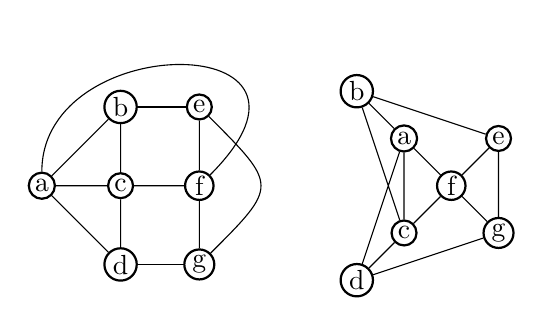
\begin{tikzpicture}[every node/.style={circle, draw, thick, inner sep=1pt}]
  \node (a) at (0,0) {a};
  \node (b) at (1,1) {b};
  \node (c) at (1,0) {c};
  \node (d) at (1,-1)  {d};
  \node (e) at (2,1) {e};
  \node (f) at (2,0) {f};
  \node (g) at (2,-1) {g};

  \draw (a) -- (b) -- (c) -- (d) -- (a) -- (c) -- (f) -- (e) .. controls (3,0) and (3,0) .. (g)--(f) .. controls (4,2) and (0,2) .. (a);
  \draw (b)--(e);
  \draw (d)--(g);

  \begin{scope}[xshift=4cm, scale=.6]
  \node (a) at (0,2) {b};
  \node (b) at (0,-2) {d};
  \node (c) at (3,1) {e};
  \node (d) at (3,-1)  {g};
  \node (e) at (1,1) {a};
  \node (f) at (1,-1) {c};
  \node (g) at (2,0) {f};

  \draw(a)--(c)--(d)--(b)--(e)--(a)--(f)--(e)--(g)--(c);
  \draw (g)--(d);
  \draw (b)--(f)--(g);
  
    \end{scope}
\end{tikzpicture}
\end{center}
  
\end{frame}

\begin{frame}{Basic graphs and concepts}
  \begin{itemize}
  \item The \emph{empty graph} $E_n$ has $n$ vertices and no edges
  \item The \emph{complete graph} $K_n$ has $n$ vertices, and each vertex is connected to every other.
  \item The \emph{path graph} $P_n$ has $n$ vertices $\{1,\dots,n\}$ with an edge between $i$ and $i+1$
    \item The \emph{cycle graph} $C_n$ has $n$ vertices $\{1,\dots, n\}$ with an edge between $i$ and $i+1$ and between $n$ and $1$.

  \end{itemize}

\begin{definition}Let $G$ be a simple graph with vertex set $V$.  Its \emph{complement} $G^c$ is another graph with vertex set $V$, where two vertices $v,w\in V$ are adjacent in $G^c$ if and only if they are not adjacent in $G$. \end{definition}
  
\end{frame}

\begin{frame}{Obligatory Petersen graph}
  \begin{center}
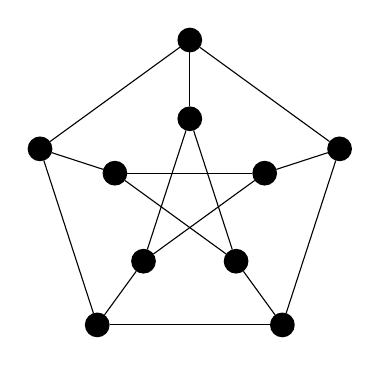
\begin{tikzpicture}[every node/.style={circle, draw, fill=black, inner sep=0pt, minimum width=4pt, thick}]
  \graph[clockwise, radius=2cm] {subgraph C_n [n=5,name=A]};
  \graph[clockwise, radius=1cm] {subgraph I_n [n=5,name=B]};

  \foreach \i in {1,2,3,4,5}{\draw (A \i) -- (B \i);}
  \newcounter{j}
  \foreach \i in {1,2,3,4,5}{%
  \pgfmathsetcounter{j}{ifthenelse(mod(\i+2,5),mod(\i+2,5),5)}
  \draw (B \i) -- (B \thej);
  }
\end{tikzpicture}
\end{center}
\end{frame}

\begin{frame}[plain,c]

\begin{center}

\Huge

\usebeamercolor[fg]{frametitle}
What does it mean for a graph to be connected?
\end{center}

\end{frame}


\begin{frame}{Connected means we can ``get from any vertex to another''}
  \begin{definition}[Walk] Let $G$ be a simple graph.  A \emph{walk} in $G$ is a sequence of vertices $v_1, v_2, \dots, v_n$ so that $v_i$ is adjacent to $v_{i+1}$.  We we say the walk goes from $v_1$ to $v_n$.
    \end{definition}

  \begin{definition}[Connected] A graph $G$ is \emph{connected} if there is a walk between any two vertices $v$ and $w$ in $G$.
  \end{definition}

  \begin{block}{Definitions I won't use without explaining}
    \begin{itemize}
    \item A \emph{trail} is a walk that doesn't repeat any edges
    \item A \emph{path} is a walk that doesn't repeat any vertices
    \end{itemize}
    \end{block}

\end{frame}
  
\begin{frame}{Bipartite graphs}
  \begin{definition}[Bipartite graphs] A graph $G$ is \emph{bipartite} if we can colour every vertex either blue or red so that every edge goes between a blue vertex and a red vertex.
  \end{definition}
  \begin{definition}[Complete bipartite graphs] The \emph{complete bipartite graph} $K_{m,n}$ consists of $m+n$ vertices, $m$ coloured red, $n$ coloured blue, and an edge between any red vertex and and any blue vertex.
  \end{definition}

  \begin{block}{Examples}
    \end{block}
\end{frame}

\begin{frame}{Another way to characterise bipartite graphs}  
  \begin{lemma}A graph $G$ is bipartite if and only if it doesn't have any cycles of odd length (i.e., subgraphs of the form $C_{2k+1}$).
    
    \end{lemma}
  \begin{block}{Bipartite $\implies$ no odd cycles:}
    Subgraphs of bipartite graphs are bipartite
  \end{block}
  \begin{block}{No odd cycles $\implies$ Bipartite:}
Try to colour $G$ by distance from $v$   
\end{block}
  \begin{definition}[Distance]Let $G$ be connected, and let $v,w$ be two vertices.  The \emph{distance from $v$ to $w$} is the least number of edges in any walk from $v$ to $w$.
    \end{definition}


  
\end{frame}




    
\end{document}
